\section{Software}
The robot will need different components of software to be able to move, map the area it is moving in, and avoid obstacles. This section will introduce the different types of software that is needed for doing as mentioned above.

\subsection{ROS}
ROS is a platform to interact with robots. This platform comes with a collection of libraries and different commands to execute the communication.\\
The idea with ROS is to connect topics to each other through nodes. On each node there is a topic that you can subscribe or publish to. When there is published or subscribed on a topic it is received in a message that contain the data of this topic. The data can then be used in different programs, to interact with the robot or get information about location and visualization. \\
Before all of this can work there is the need for ROS-master. The ROS-master keeps track of every topic that has been subscribed or published to.

\subsection{Rviz}
Rviz is a program used by ROS to provide 3D images and point clouds from data given by the robots sensors. Rviz lets us see what the robot is seeing and doing. The input the robot gets from cameras and sensors is just numbers and coordinates and Rviz converts these numbers into 3D objects which represent these objects\cite{interactiveMarkers}.

\subsection{Mapping}
ROS has a mapping package called gmapping. The gmapping package provides laser-based SLAM, as a ROS node called slam\_gmapping. Furthermore, slam\_gmapping creates a 2D map in Rviz (like building a floor plan) with lasers and position data collected by a robot\cite{mapping}.

\subsection{Localization}
Robot localization is a task to move safely from one location to another.
It helps determine a  Turtlebot position by using an adaptive Monte Carlo localization approach (AMCL). The localization system AMCL is collecting information from the sensors such as odometry.\\By comparing data from sensors to the known map, it is possible to estimate the current position of the robot.\\In Rviz created visual maps, the robot find the trajectory to move forward. The two processes are commonly referred to as SLAM. A localization system, AMCL, working process is described in figure \ref{fig:amcl}.

\begin{figure}[h]
    \centering
    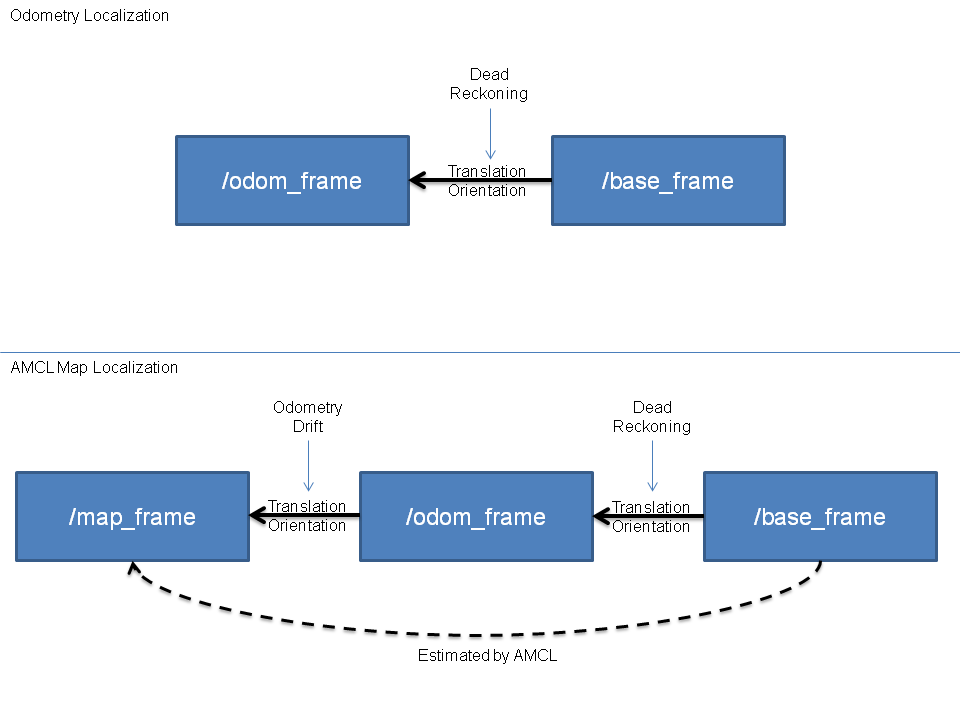
\includegraphics[width=.7\textwidth]{figures/AMCL.png}
    \caption{AMCL working process\cite{AMCL}} 
    \label{fig:amcl} 
\end{figure}

 During operation AMCL estimates the transformation of the base frame in respect to the global frame but it only publishes the transform between the global frame and the odometry frame\cite{AMCL}.

\subsection{SLAM}
SLAM is not a specific algorithm, but a concept where there are many different approaches. SLAM use a collection of data gathered from various measuring sensors, to build a map and to triangulate itself inside this map.
There are different solutions for SLAM some are made for indoor use some for outdoor, and some is made to navigate in an area with terrain.\\
When the robot starts mapping, it will then look with its sensors, LIDAR, laser, etc. for objects. After the robot moves forward, it measures how far it has moved with the odometry sensor and gyroscope, then looks at the surrounding area to check its new relative position with objects\cite{SLAMdummies}\cite{DifferentSLAM}\cite{GyrosOdometry}.\\
%A simple algorithm for SLAM could be:
%\begin{itemize}
%    \item Scan area for objects
%    \item Move forward and measure how far
%    \item Scan again for objects
%    \item Look for reappearing objects
%    \item Triangulate location to objects that reappeared
%    \item Relocate the robot in the map 
%\end{itemize}

\subsection{Frontier Exploration}


